\section{The ATLAS detector}
\label{sec:ATLAS}
\begin{comment}


\begin{itemize}
    \item Skriv kort om ATLAS
    \item Tracking
    \item luminositet osv
    \item luminosity $10^{34} cm^{-2}s^{-1}$ for proton-proton
    \item upgrade to HL-LHC
    \item size
    \item figure of tracks
    \item coordinate system and navngiving og nyttige variabler: lumi og pileup og number of interations and rate.
    \item origin of the coordinate system: nominal interaction point
    \item $\phi$ og $\Theta$
    \item transverse og alle er definert i x-y-planet
    \item pseudo rapidity
    \item $\Delta R_{ll}$
    \item INNER DETECTOR:
    \item Hvor den er
    \item Exposed for mye radiation og derfor må vi oppgradere nå
    \item scheduled at 2024, men vil bli utsatt (som er neste oppgradering igjen)
    \item Tracker de første bevegelsene av partiklene som er skapt i kollisjonen og må være veldig presis. 
    \item inner detector er inni et 2T magnetfelt som kommer fra the central solenoid. Som er med på å hjelpe oss å tracke partikler fordi ladde partikler vil bendes av mahnetfeltet.
    \item bilde av inner detector
    \item CALORIMETERS:
    \item Du må vite energien for å rekonsturere partikler fra kollisjonen. Calorimeteret måler hvor mye energi partikkelen legger igjen når den møter detektormaterialet.
    \item To er brukt: one EM calorimeter og hadronic calorimeter
    \item Bilde av begge calorimeters (en figur)
    \item Vi trenger calorimeters for å tracke ET og det er viktig for BSM.
    \item EM cal:
    \item for å tracke electrons og photons 
    \item HAD cal:
    \item Outside of EM og den er bygd for å tracke hadrons og hadronic showers. Legg in hva en shower er. cascade decay.
    \item jet reconstruction og met
    \item MAGNETS:
    \item ATLAS består av to magnetsystemer: a central solenoid og a barrel (symmetrisk rundt beam axis) toreoid og two end-cap toreoids. 
    \item MUON system:
    \item basert på magnet deflection of muon tracks. Muon kammerne eksisterer rundt hele detektoren hvor den går rundt beam aksen og de ytterste ligger i x-y-planet. Ligger som en tønne rundt beam aksen og med lokk på endene. barrel region og end-cap regions.
    \item Triggers and data acquesition? 
    
\end{itemize}
\end{comment}


The ATLAS \cite{ATLAS} detector is a massive 44 m long detector, 25 m in diameter and weighing about the same as the Eiffel tower ($\sim 7000$ tons). It is designed to handle proton-proton collisions up to 14 TeV with a luminosity of a few times $10^{34}$cm$^{-2}$s$^{-1}$. We can see an illustration of the whole detector in figure \ref{fig:atlas}, where the most important components are marked. 


\begin{figure}[H]
    \centering
    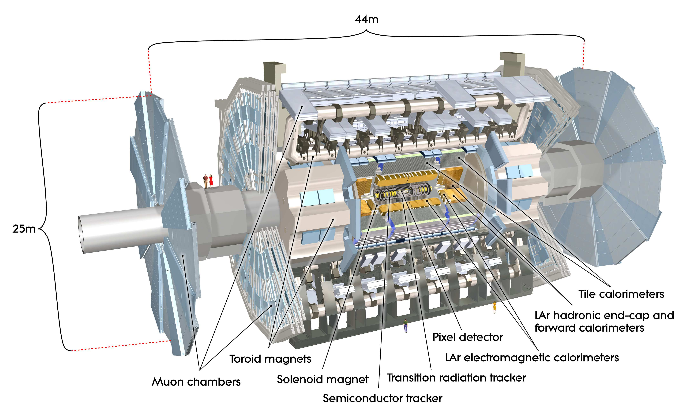
\includegraphics[width = \textwidth]{Figures/FromOnline/ATLAS.png}
    \caption{An illustration of the ATLAS detector \cite{ATLAS}.}
    \label{fig:atlas}
\end{figure}

The detector is built up of three main layers. Two inner tracking layers, that provide the information about particle trajectories and allow to determine, with good resolution, the interaction point and secondary vertices\footnote{Secondary vertices is the interaction vertices for particles that decay after the collision or collide into decays from other collisions.}. The inner detector is composed of a pixel and strip silicon tracker and a transition radiation tracker. A good tracking resolution is in fact needed for particle track momentum determination and primary and secondary vertex measurement purposes: the whole inner detector is inserted in a solenoid magnet that generates a magnetic field along the beam direction. The bending trajectory of charged particles in magnetic field leads to a determination of momentum and electric charge of the particles.

The tracker is followed by two layers of calorimeters. The innermost is the electromagnetic calorimeter and consists of alternating layers of lead and liquid argon. The purpose of the layer is to stop incoming photons, positrons and electrons by inducing electromagnetic showers that allow to measure the energy of these particles. The outer calorimeter is the hadronic calorimeter, composed of three different parts. The hadrons produced in the event interact with the calorimeter material and produce hadronic showers, also called \textit{jets}, which lose their whole energy in the hadronic calorimeter. 

The outer layer consists of the muon chambers, which surround the whole detector as a barrel with two end-caps at the edges. Muons are the only detectable particles that are able to travel through all the other layers, only depositing a minimum ionisation energy in the detector material along the trajectory. 

All the particles we can not track in the detector layers are referred to as missing energy/momentum, essentially inferred from energy-momentum conservation and the measurement of all visible particle energy and momenta $E_{miss} = -\sum_i E_i$ and $\Vec{p}_{miss} = -\sum_i \Vec{p}_i$. 

A sketch of the sub-detector layers presented above is shown in figure \ref{fig:tracks}.

\begin{figure}[H]
    \centering
    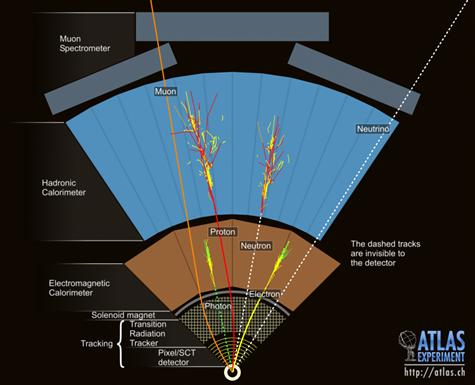
\includegraphics[width = 0.8\textwidth]{Figures/FromOnline/tracks.jpg}
    \caption{An illustration on how we see the tracks of the different particles in the detector \cite{tracks}.}
    \label{fig:tracks}
\end{figure}


\subsection{Kinematic variables and the ATLAS coordinate system}
By combining information from the different sub-detector layers it is possible to calculate various kinematical variables and identify the different particle species. In the beam direction, corresponding to the z-axis. We have two protons with opposite momenta $p$ in each collision and therefore we are interested mostly in the transverse direction, where energy and momentum is conserved. The energy deposited by the particle is measured by the calorimeter and combined with the tracking information to have the vector quantities of $p_T$ and $E_T$ connected by the invariant mass m of the particle by the relation $p_T^2 = E_T^2 - m^2$. As mentioned before we can measure the difference in the transverse energy before and after the collision, which gives us the \textit{missing transverse energy} (MET/$E_T^{miss}$). 

It is also useful to introduce the detector coordinates used to describe an event. A sketch is shown in figure \ref{fig:coordsys}. The $z$-coordinate is defined by the beam direction and the $x,y$-coordinates define the transverse plane. In addition we have the two angles $\theta$ (polar) and $\phi$ (azimuthal), being the angle between the particle and the $z$-axis and the particle and the $x$-axis, respectively. Note that instead of referring to the coordinate $\theta$ it is common to introduce the pseudorapidity $\eta$ defined as 

\begin{equation}
    \eta = -\ln \tan \bigg(\frac{\theta}{2}\bigg).
\end{equation}

\begin{figure}[H]
    \centering
    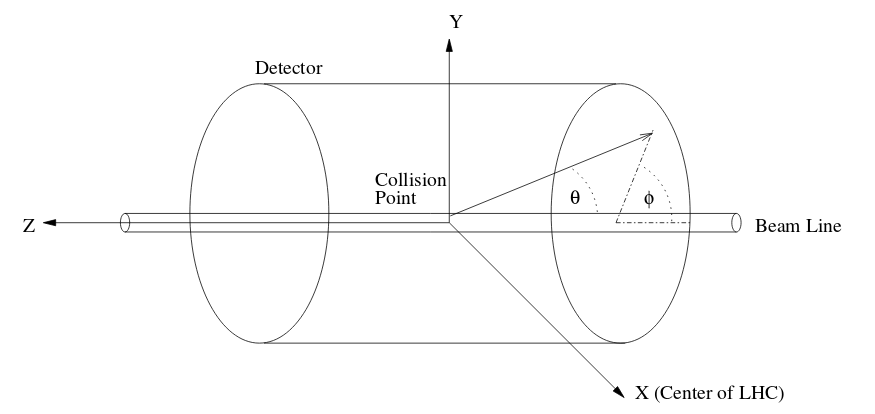
\includegraphics[width = \textwidth]{Figures/FromOnline/coordinatesystem.png}
    \caption{An illustration of the coordinate system inside the detector\cite{coordinatesystem}.}
    \label{fig:coordsys}
\end{figure}

The other variables we are considering in this thesis, where we are interested in final states with two leptons $l^+ l^-$ and missing transverse momentum and energy, are listed below

\begin{itemize}
    \item $m_{l^+l^-}$ is the invariant mass of the lepton pair in the final state, defined as 
            \begin{equation}
                m_{l^+l^-} = \sqrt{(E_{l^+} + E_{l^-})^2 - (\mathbf{p}_{l^+} + \mathbf{p}_{l^-})^2}.
            \end{equation}
            
    \item $m_{T2}$, transverse mass defined as 
            \begin{equation}
                \label{eq:mt}
                m_T = \sqrt{2 |\mathbf{p}_{T,1}| \cdot |\mathbf{p}_{T,2}| \cdot \big(1-\cos(\Delta\phi)\big)},
            \end{equation}
        where $\mathbf{p}_{T,1}$ and $\mathbf{p}_{T,2}$ are the transverse momentum vectors of the two leptons in the final state and $\Delta \phi$ is defined below.
    \item $m_{T2}$ is the stransverse mass \cite{Lester:1999tx, Barr:2003rg} and is used to describe the masses of a particle pair that is assumed to have decayed to one visible and one invisible particle. It is defined as 
    \begin{equation*}
        m_{T2}(\mathbf{p}_{T,1}, \mathbf{p}_{T,2}, \mathbf{p}_{T}^{miss}) = \min_{q_{T,1} + q_{T,2} = p_T^{miss}} \bigg\{\max\big[m_T(\mathbf{p}_{T,1}, \mathbf{q}_{T,1}), m_T(\mathbf{p}_{T,2}, \mathbf{q}_{T,2})\big]\bigg\},
    \end{equation*}
    where $m_T$ is the transverse mass defined in equation \ref{mt} and $\mathbf{q}_{T,1}$ and $\mathbf{q}_{T,2}$ are vectors with $\mathbf{p}_{T}^{miss} = \mathbf{q}_{T,1} + \mathbf{q}_{T,2}$. 
    \item  $H_T$ is the scalar sum of the $p_T$ of the leptons we have selected and of the jets in the event.
    \item  $\Delta \phi (\Vec{p}_T^{ll}, E_T^{miss})$ is the difference between the azimuthal angles of the two-lepton system and the missing transverse energy direction.
    \item $\Delta R_{ll} = \sqrt{(\Delta\phi_{ll})^2 + (\Delta \eta_{ll})^2}$ is the distance between the two leptons in the final ($\phi, \eta$) plane.
\end{itemize}


   
  
    







\begin{comment}


\begin{figure}[H]
    \centering
    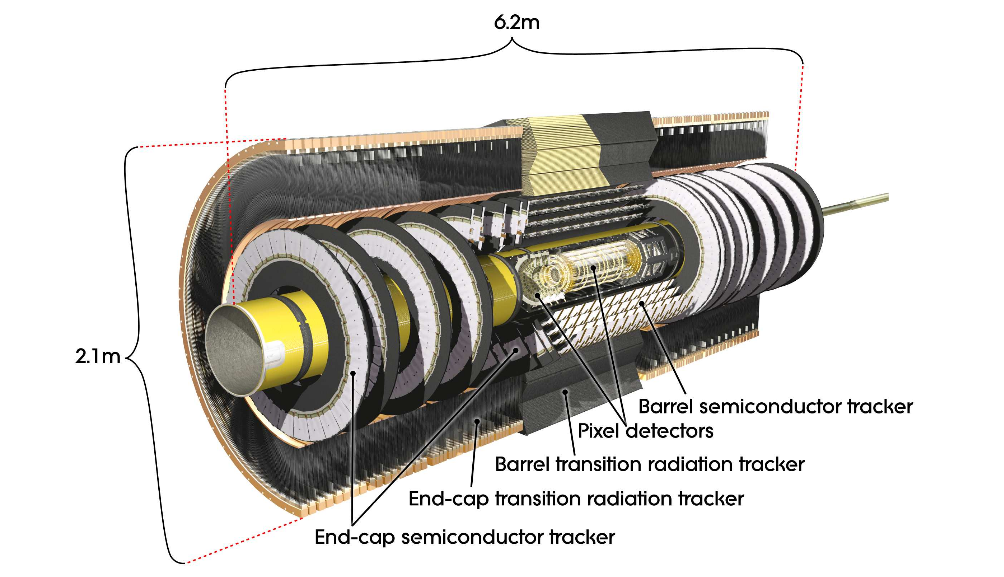
\includegraphics[width = \textwidth]{Figures/FromOnline/innerdetector.png}
    \caption{An illustration of the inner detector \cite{innerdetector}.}
    \label{fig:innerdet}
\end{figure}


\begin{figure}[H]
    \centering
    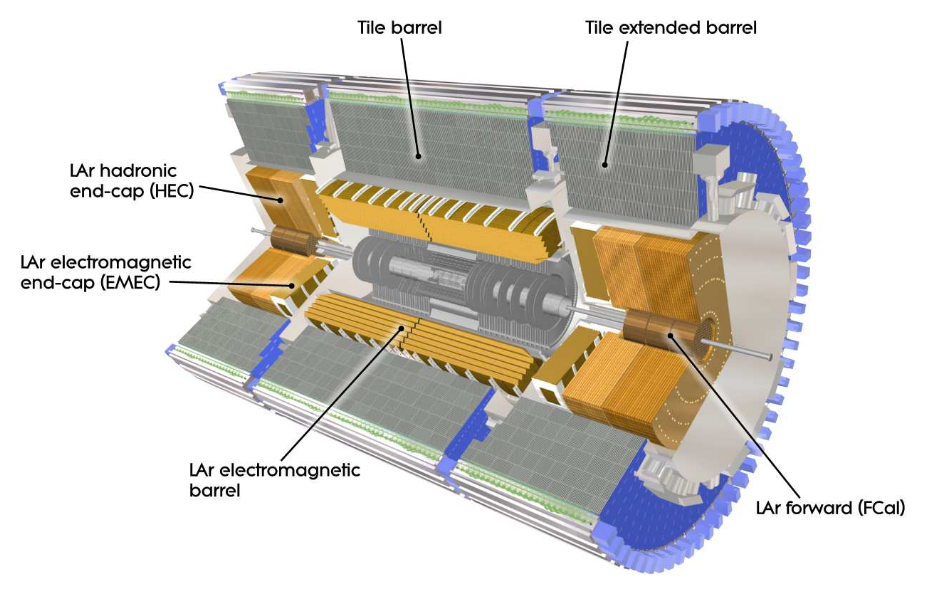
\includegraphics[width = \textwidth]{Figures/FromOnline/calorimeters.png}
    \caption{An illustration of the calorimeters \cite{innerdetector}.}
    \label{fig:calori}
\end{figure}


\begin{figure}[H]
    \centering
    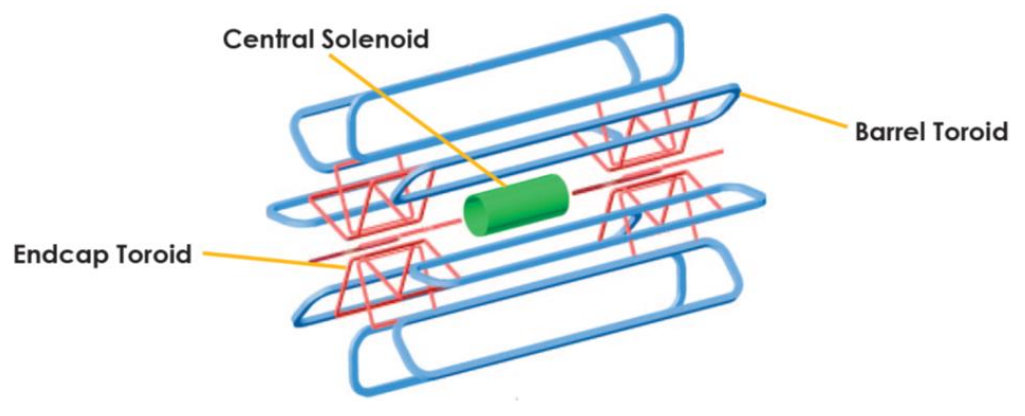
\includegraphics[width = \textwidth]{Figures/FromOnline/magnetsystem.png}
    \caption{An illustration of the magnet systems \cite{magnetsystem}.}
    \label{fig:magnetsys}
\end{figure}
\end{comment}















